\newpage
\appendix
\section{Hyperparameter search}\label{ap:hyperparam}
\begin{figure}[!h]
    \centering
    \begin{tabular}{@{}c@{}}
        \includegraphics[width=\linewidth]{images/hyperparam20.png}
    \end{tabular}
    % \vspace{-1em}
    \begin{tabular}{@{}c@{}}
        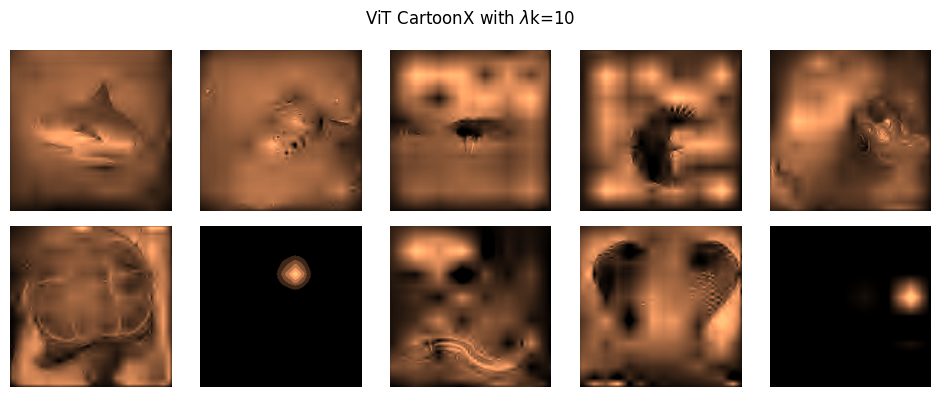
\includegraphics[width=\linewidth]{images/hyperparam10.png}
    \end{tabular}
    % \vspace{-1em}
    \begin{tabular}{@{}c@{}}
        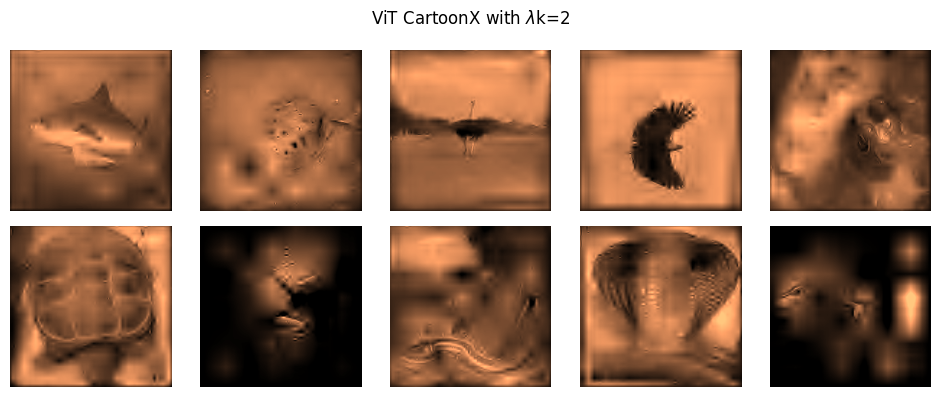
\includegraphics[width=\linewidth]{images/hyperparam2.png}
    \end{tabular}
    \caption{Ten examples of CartoonX with a ViT with $\lambda k = 2, 10, 200$ are depicted in the two top, middle and bottom rows, respectively. Overall, with $\lambda k = 20$, most of the explanations are relatively sparse, with some explanations being completely black. With $\lambda k = 2$ there are no entirely black explanations. However, with this setting some explanations of images did not contain a lot of sparsity, i.e. did not show a clear explanation. Utilising  $\lambda k = 10$ constituted a suitable trade‐off between the explanations' sparsity and their expressiveness for most images.}
    \label{fig:hyperparamsVit}
\end{figure}
